\documentclass[tikz,border=10pt]{standalone}
\usepackage{tikz}
\usepackage{xcolor}
\usetikzlibrary{shapes,arrows,positioning,fit,backgrounds,decorations.pathmorphing}

% Define colors
\definecolor{flblue}{RGB}{70,130,180}
\definecolor{rlgreen}{RGB}{34,139,34}
\definecolor{cacheorange}{RGB}{255,140,0}
\definecolor{lightgray}{RGB}{240,240,240}
\definecolor{darkgray}{RGB}{128,128,128}

\begin{document}
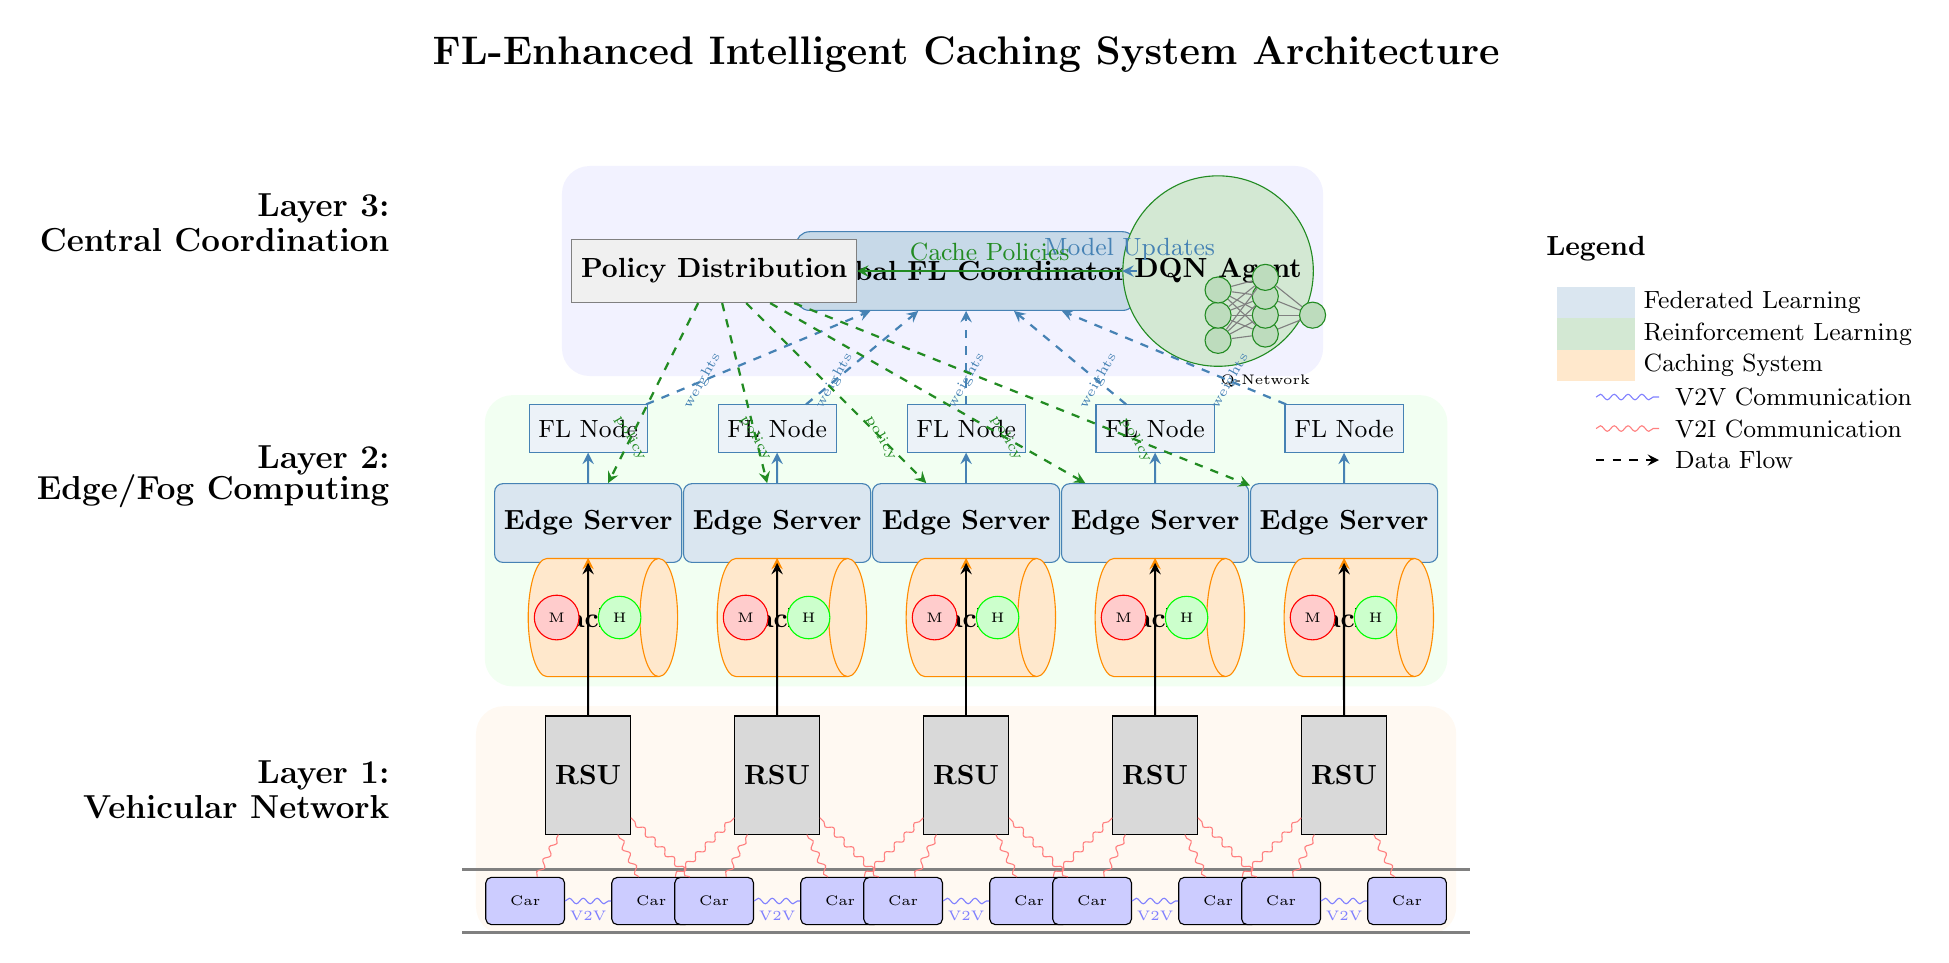
\begin{tikzpicture}[
    node distance=1.5cm,
    vehicle/.style={rectangle, draw=black, fill=blue!20, minimum width=1cm, minimum height=0.6cm, rounded corners=2pt},
    rsu/.style={rectangle, draw=black, fill=gray!30, minimum width=0.8cm, minimum height=1.5cm},
    edge/.style={rectangle, draw=flblue, fill=flblue!20, minimum width=2cm, minimum height=1cm, rounded corners=3pt},
    cache/.style={cylinder, draw=cacheorange, fill=cacheorange!20, minimum width=1.5cm, minimum height=0.8cm},
    brain/.style={circle, draw=rlgreen, fill=rlgreen!20, minimum size=1.2cm},
    coordinator/.style={rectangle, draw=flblue, fill=flblue!30, minimum width=3cm, minimum height=1cm, rounded corners=5pt},
    arrow/.style={->, >=stealth, thick},
    wireless/.style={decorate, decoration={snake, amplitude=1pt, segment length=5pt}},
    scale=0.8
]

% Title
\node[above] at (0,12) {\Large\textbf{FL-Enhanced Intelligent Caching System Architecture}};

% Layer 3: Central Coordination Layer
\begin{scope}[yshift=9cm]
    \node[coordinator] (global_fl) at (0,0) {\textbf{Global FL Coordinator}};
    \node[brain] (dqn) at (4,0) {\textbf{DQN Agent}};
    \node[rectangle, draw=darkgray, fill=lightgray, minimum width=2cm, minimum height=0.8cm] (policy) at (-4,0) {\textbf{Policy Distribution}};
    
    % Neural network representation
    \begin{scope}[xshift=4cm, yshift=-1.5cm, scale=0.5]
        \foreach \i in {1,2,3} {
            \node[circle, draw=rlgreen, fill=rlgreen!30, minimum size=0.3cm] (input\i) at (0,\i*0.8) {};
        }
        \foreach \i in {1,2,3,4} {
            \node[circle, draw=rlgreen, fill=rlgreen!30, minimum size=0.3cm] (hidden\i) at (1.5,\i*0.6+0.4) {};
        }
        \node[circle, draw=rlgreen, fill=rlgreen!30, minimum size=0.3cm] (output) at (3,1.6) {};
        
        \foreach \i in {1,2,3} {
            \foreach \j in {1,2,3,4} {
                \draw[gray, thin] (input\i) -- (hidden\j);
            }
        }
        \foreach \i in {1,2,3,4} {
            \draw[gray, thin] (hidden\i) -- (output);
        }
        \node[below] at (1.5,0) {\tiny Q-Network};
    \end{scope}
    
    \draw[arrow, flblue] (global_fl) -- (dqn) node[midway, above] {\small Model Updates};
    \draw[arrow, rlgreen] (dqn) -- (policy) node[midway, above] {\small Cache Policies};
\end{scope}

% Layer 2: Edge/Fog Computing Layer
\begin{scope}[yshift=5cm]
    \foreach \x in {-6,-3,0,3,6} {
        \node[edge] (edge\x) at (\x,0) {\textbf{Edge Server}};
        \node[cache] (cache\x) at (\x,-1.5) {\textbf{Cache}};
        \node[rectangle, draw=flblue, fill=flblue!10, minimum width=1.5cm, minimum height=0.6cm] (fl\x) at (\x,1.5) {\small FL Node};
        
        \draw[arrow, cacheorange] (edge\x) -- (cache\x);
        \draw[arrow, flblue] (edge\x) -- (fl\x);
        
        % Cache hit/miss indicators
        \node[circle, draw=green, fill=green!20, minimum size=0.3cm] (hit\x) at (\x+0.5,-1.5) {\tiny H};
        \node[circle, draw=red, fill=red!20, minimum size=0.3cm] (miss\x) at (\x-0.5,-1.5) {\tiny M};
    }
    
    % FL aggregation arrows
    \foreach \x in {-6,-3,0,3,6} {
        \draw[arrow, flblue, dashed] (fl\x) -- (global_fl) node[near start, rotate=60] {\tiny weights};
    }
    
    % Policy distribution arrows
    \foreach \x in {-6,-3,0,3,6} {
        \draw[arrow, rlgreen, dashed] (policy) -- (edge\x) node[near end, rotate=-60] {\tiny policy};
    }
\end{scope}

% Layer 1: Vehicular Network Layer
\begin{scope}[yshift=1cm]
    % RSUs
    \foreach \x in {-6,-3,0,3,6} {
        \node[rsu] (rsu\x) at (\x,0) {\textbf{RSU}};
        \draw[arrow, thick] (rsu\x) -- (edge\x);
    }
    
    % Vehicles
    \foreach \x in {-7,-5,-4,-2,-1,1,2,4,5,7} {
        \node[vehicle] (car\x) at (\x,-2) {\tiny Car};
    }
    
    % Roads
    \draw[thick, gray] (-8,-2.5) -- (8,-2.5);
    \draw[thick, gray] (-8,-1.5) -- (8,-1.5);
    
    % V2V communications
    \foreach \x in {-7,-4,-1,2,5} {
        \pgfmathtruncatemacro{\next}{\x+2}
        \draw[wireless, blue!50] (car\x) -- (car\next) node[midway, below] {\tiny V2V};
    }
    
    % V2I communications
    \foreach \x in {-6,-3,0,3,6} {
        \foreach \y in {-7,-5,-4,-2,-1,1,2,4,5,7} {
            \pgfmathparse{abs(\x-\y)}
            \ifdim\pgfmathresult pt<2.5pt
                \draw[wireless, red!50] (car\y) -- (rsu\x);
            \fi
        }
    }
\end{scope}

% Layer labels
\node[left, font=\large\bfseries] at (-9,10) {Layer 3:};
\node[left, font=\large\bfseries] at (-9,9.5) {Central Coordination};

\node[left, font=\large\bfseries] at (-9,6) {Layer 2:};
\node[left, font=\large\bfseries] at (-9,5.5) {Edge/Fog Computing};

\node[left, font=\large\bfseries] at (-9,1) {Layer 1:};
\node[left, font=\large\bfseries] at (-9,0.5) {Vehicular Network};

% Legend
\begin{scope}[xshift=10cm, yshift=6cm]
    \node[above] at (0,3) {\textbf{Legend}};
    
    \node[flblue, fill=flblue!20, minimum width=1cm, minimum height=0.4cm] at (0,2.5) {};
    \node[right] at (0.6,2.5) {\small Federated Learning};
    
    \node[rlgreen, fill=rlgreen!20, minimum width=1cm, minimum height=0.4cm] at (0,2) {};
    \node[right] at (0.6,2) {\small Reinforcement Learning};
    
    \node[cacheorange, fill=cacheorange!20, minimum width=1cm, minimum height=0.4cm] at (0,1.5) {};
    \node[right] at (0.6,1.5) {\small Caching System};
    
    \draw[wireless, blue!50] (0,1) -- (1,1);
    \node[right] at (1.1,1) {\small V2V Communication};
    
    \draw[wireless, red!50] (0,0.5) -- (1,0.5);
    \node[right] at (1.1,0.5) {\small V2I Communication};
    
    \draw[arrow, dashed] (0,0) -- (1,0);
    \node[right] at (1.1,0) {\small Data Flow};
\end{scope}

% Background boxes for layers
\begin{scope}[on background layer]
    \node[fill=blue!5, rounded corners=10pt, fit={(policy) (dqn) (global_fl)}] {};
    \node[fill=green!5, rounded corners=10pt, fit={(fl-6) (fl6) (edge-6) (edge6) (cache-6) (cache6)}] {};
    \node[fill=orange!5, rounded corners=10pt, fit={(rsu-6) (rsu6) (car-7) (car7)}] {};
\end{scope}

\end{tikzpicture}
\end{document}
